\chapter{Beszélőazonosító rendszerek napjainkban}

A fejezet bemutatja a tanítás során használt beszédadatbázisokat, két neurális hálózat alapú, zárt-halmazú, automatikus beszélőfelismerő rendszert; a \emph{WaveNet classifiert} és a \emph{SincNetet} illetve az ezekkel elért eredményeket.

\section{Beszédadatbázisok}

\subsection{TIMIT}

A TIMIT beszédkorpuszt automatikus beszédfelismerő rendszerek fejlesztéséhez tervezték. 630 beszélőtől tartalmaz mintákat amerikai angol nyelven a 8 legelterjedtebb nyelvjárásban.
A TIMIT archívum tartalmaz egy TRAIN és egy TEST mappát, ezek tanításhoz és teszteléshez valók. Ezeken belül további, a dialektusok sorszámával (DR1, ..., DR8), azon belül a beszélő azonosítójával elnevezett könyvtárak találhatók. Egy beszélőhöz
10 db beszédminta tartozik 16 kHz-es NIST SPHERE fájlok formájában.


\begin{table}[!ht]
	\begin{tabular}{*4l} \toprule
		\bfseries Dialektus regió (DR) & \bfseries Férfi & \bfseries Nő & \bfseries Összesen \\ \midrule
		1                             & 31 (63\%)      & 18 (27\%)   & 49 (8\%)          \\
		\rowcolor{gray!10} 
		2                             & 71 (70\%)      & 31 (30\%)   & 102 (16\%)        \\
		3                             & 79 (67\%)      & 23 (23\%)   & 102 (16\%)        \\
		\rowcolor{gray!10} 
		4                             & 69 (69\%)      & 31 (31\%)   & 100 (16\%)        \\
		5                             & 62 (63\%)      & 36 (37\%)   & 98 (16\%)         \\
		\rowcolor{gray!10} 
		6                             & 30 (65\%)      & 16 (35\%)   & 46 (7\%)          \\
		7                             & 74 (74\%)      & 26 (26\%)   & 100 (16\%)        \\
		\rowcolor{gray!10} 
		8                             & 22 (67\%)      & 11 (33\%)   & 33 (5\%)          \\
		\bottomrule
		\hline
	\end{tabular}
	\centering
	\caption{A beszélők eloszlása dialektusok szerint.}
	\label{fig:timit-dialects}
\end{table}

A dialektus régiók a következők:

\begin{multicols}{2}
	\begin{itemize}
		\item DR1:  New England
		\item DR2:  Northern
		\item DR3:  North Midland
		\item DR4:  South Midland
		\item DR5:  Southern
		\item DR6:  New York City
		\item DR7:  Western
		\item DR8:  Army Brat (moved around)
	\end{itemize}
\end{multicols}

A NIST SPHERE formátum az elején definiál egy fix hosszú fejlécet, amit a hang bináris kódolása követ. Erre figyelni kell a hangfájlok beolvasásánál, Python esetében nem minden hangfeldolgozó könyvtár támogatja. Ilyen esetben kézzel el kell távolítani a fejlécet a fájlok elejéről. A hangfájlokhoz tartozik egy szöveges dokumentum ami az elhangzott szöveget és annak a wav fájlbeli helyét tartalmazza. Továbbá egy WRD fájl írja le a szavakat és egy PHN kiterjesztésű a fonémákat, illetve azok időbeni elhelyezkedését a wav fájlban.

A hangfájlokhoz tartozó egyéb fájlok beszédfelismerés szempontjából fontosak. Mivel én a beszédkorpuszt beszélőfelismerésre használtam, csak a hangfájlokra volt szükségem. A TEST mappában - mivel a TIMIT-et alapvetően beszédfelismeréshez tervezték - teljesen különböző beszélők vannak a TRAIN mappához képest, ezért a TRAIN mappabeli beszélőket kell felosztani tanításhoz és teszteléshez.

\subsection{CMU Arctic}

A CMU Arctic beszédadatbázist beszédszintézis kutatásokhoz tervezték. 18 adathalmazt tartalmaz 18 különböző embertől más-más akcentussal, angol nyelven. Egy emberhez több száz beszédminta tartozik wav fájlok formájában.

\subsection{Adatok előfeldolgozása}

Az előfeldolgozó szkript a TIMIT adatbázis esetében a hangmintákról eltávolítja a NIST Sphere fejlécet és a mondat előtti és utáni szüneteket. Ezután normalizálja a hangmintákat. A CMU Arctic esetében a hangminták alapból normalizálva vannak, ezért csak azonos méretűre kell vágni őket az egységes bemeneti dimenziók érdekében (ahogy a TIMIT esetében is).

\section{Mérési elrendezés}

Google Colab...

\section{WaveNet classifier}

A \emph{WaveNet classifier} egy módosított WaveNet architektúra beszélőidentifikációhoz.

\subsection{WaveNet}

A WaveNet egy mély neurális hálózat audio hullámformák generálásához, amelyet a Google DeepMind publikált 2016-ban. Az ötletet az akkori felfedezések adták neurális autoregresszív generatív modellezés terén, amelyeket komplex eloszlások, például képek modellezésére használtak (van den Oord et al., 2016a;b). Ezt felhasználva audio hullámformák generálásában új eredményeket értek el.

\begin{itemize}
	\item Képes olyan természetes hangzású beszéd hullámformák generálására, amit korábban parametrikus vagy konkatenatív beszédszintézissel sosem értek el. 
	\item Az audio hullámformák generáláshoz szükséges nagy receptív mezőt hatékonyan, nyújtott kauzális konvolúciókkal implementálja.
	\item Ha a modellt a beszélők identitásával tanítják, képes új hangok generálására.
	\item A zene generálás és a beszédfelismerés terén is ígéretesnek bizonyult.
\end{itemize}

\subsubsection{Nyújtott kauzális konvolúció}

A modell autoregresszív, vagyis a kimenete korábbi időpillanatokban felvett értékeitől függ. Ez azért fontos, mert a WaveNet egy generatív modell. A generált hullámforma \emph{t}-edik időpillanatbeli értéke nem függhet jövőbeli értékektől. A kauzalitás legegyszerűbb implementációja ha legalább a \emph{kernel-1} méretű paddinget adunk a konvolúcióhoz.

\begin{figure}[!ht]
	\centering
	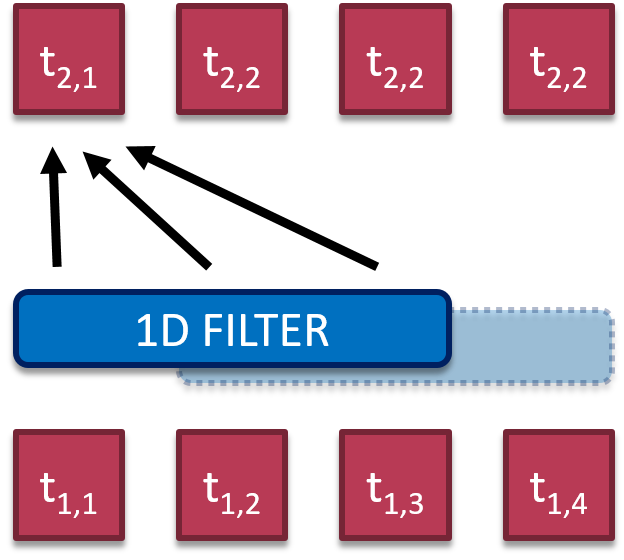
\includegraphics[width=80mm, keepaspectratio]{figures/1d-conv.png}
	\caption{1D nem kauzális konvolúció.}
	\label{fig:1d_noncausal_conv}
\end{figure}

\begin{figure}[!ht]
	\centering
	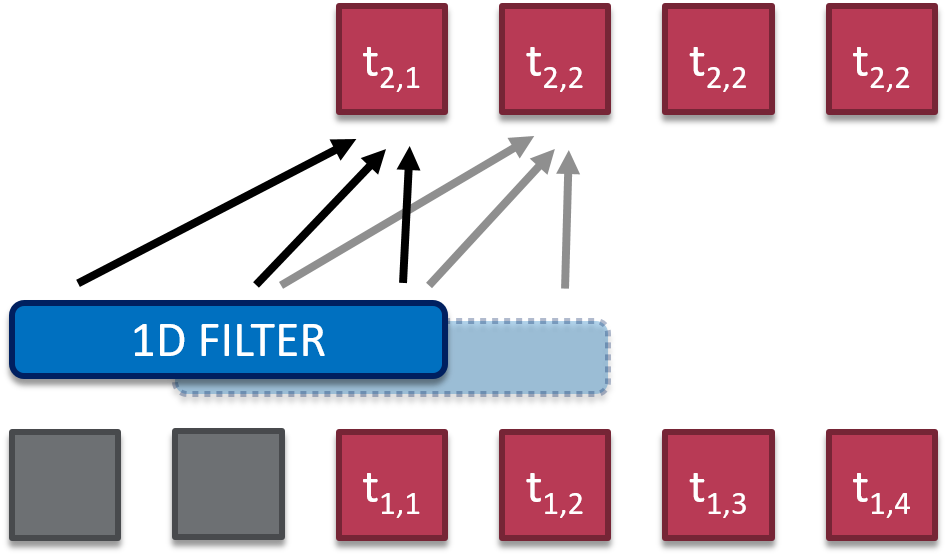
\includegraphics[width=120mm, keepaspectratio]{figures/1d-causal-conv.png}
	\caption{1D kauzális konvolúció paddinggel.}
	\label{fig:1d_causal_conv}
\end{figure}

\newpage

A \ref{fig:1d_noncausal_conv} ábra egy nem kauzális 1D konvolúciót mutat. A $t_{i, j}$ az i-edik rétegbeli j-edik neuron. Látható, hogy a $t_{2,1}$ jövőbeli időpillanatokból kap értékeket a szűrőn keresztül. Ennek megoldása a szűrő eltolása padding segítségéve. Ezt szemlélteti a \ref{fig:1d-causal-conv} ábra, ahol az egyes neuronok csak korábbi időpillanatokból kapnak értékeket. 

A beszéd generálásánál a \emph{t}-edik időpillanatban a hullámforma értéke a korábbi adatoktól függ. Ahhoz, hogy magas frekvenciájú, pl. 16 kHz frekvencián mintavételezett 
hangadattal tanítsuk a hálózatot nagy receptív mezőre van szükség. A receptív mező az a szélesség, amit a szűrő lát a bemenetből. 16 kHz esetén egy másodpercnyi jelet 16000 szám reprezentál. Ahhoz, hogy a hálózat helyesen jósolja meg a következő generált értéket, a hosszú távú dependenciákat figyelembe kell vennie, tehát a receptív mező méretét elég nagyra kell megválasztani. A probléma ekkora mezők esetén, hogy sok konvolúciós réteget igényelnek (egy korábbi időpillanatbeli adat plusz egy konvolúciós réteget igényel), ami növeli a számítási komplexitást. A nyújtott konvolúciók erre adnak hatékony megoldást. A filter meghatározott távolságokkal kihagy valamennyi inputot, majd figyelembe vesz egyet. Egymás utáni rétegekben a nyújtási tényezőt exponenciálisan növelve a receptív mező is exponenciálisan fog nőni.

\begin{figure}[!ht]
	\centering
	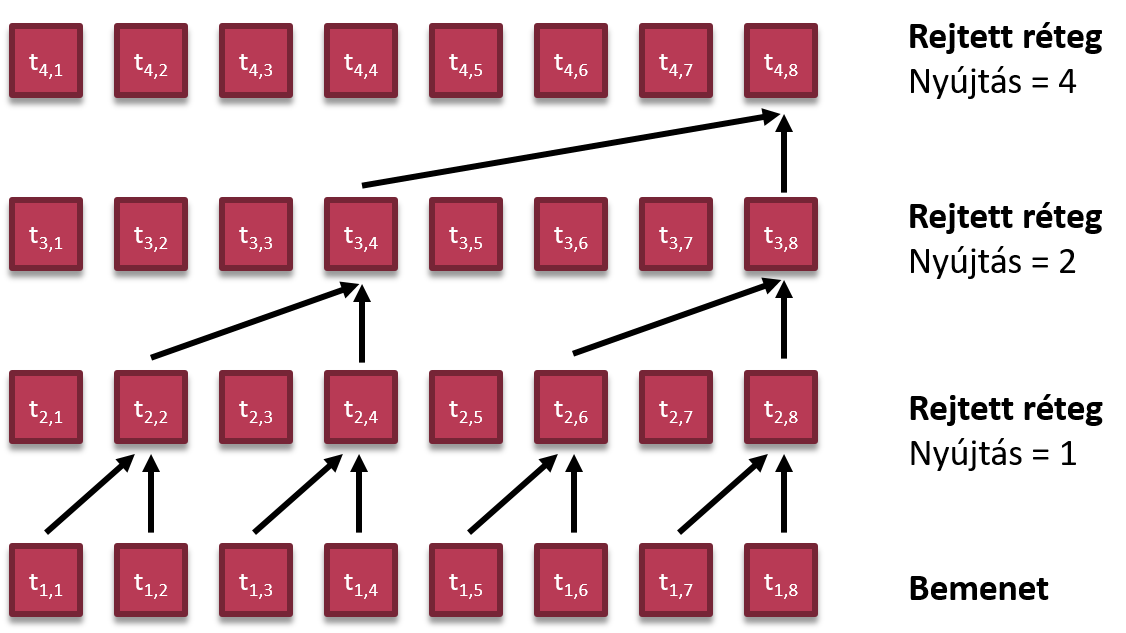
\includegraphics[width=150mm, keepaspectratio]{figures/1d-dilated-conv.png}
	\caption{1D nyújtott kauzális konvolúciós rétegek.}
	\label{fig:1d_dilated_conv}
\end{figure}

\subsubsection{SoftMax eloszlás}
A WaveNet SoftMax réteget használ a $p(x_t|x_1,\dots,x_t)$ feltételes valószínűségi eloszlás modellezésére.
Az audio jeleket általában 16 bites egészekkel kódolják, amelyek 65536 értéket vehetnek fel. Ebben az esetben a SoftMax rétegnek 65536 valószínűséget kell kimenetként adnia, melyek összege 1. A $\mu$-law kvantálást alkalmazva a beszédjel 256 biten kódolható és később az inverz transzformációval jó minőségben visszaállítható.

Az emberi hallás sokkal érzékenyebb alacsony amplitúdójú hangok kvantálási zajára, mint a magasabbakéra. Erre alapozva a $mu$-law kvantáló a jelet egy logaritmikus függvénnyel kvantálja úgy, hogy az alacsonyabb amplitúdójú jelek nagyobb felbontással (több bittel), a magasabbak pedig kisebbel lesznek kódolva. Ez növeli a SoftMax réteg hatékonyságát is, mert nagyobbak lesznek a valószínűségek közötti különbségek.

A tanítást a WaveNet klasszifikációs problémaként kezeli. A bemeneteket OneHot kódolással adjuk meg, a SoftMax réteg pedig az így kódolt egészekre ad valószínűségi eloszlást.

\subsubsection{Reziduális blokkok}

A WaveNet architektúra egymáshoz csatolt reziduális blokkokból és ún. kapcsolat-ugrásokból (skip-connection) épül föl. A reziduális hálózatok előnye, hogy orvosolják az elenyésző gradiens problémát, így sokkal mélyebb hálózat építhető.

\begin{figure}[!ht]
	\centering
	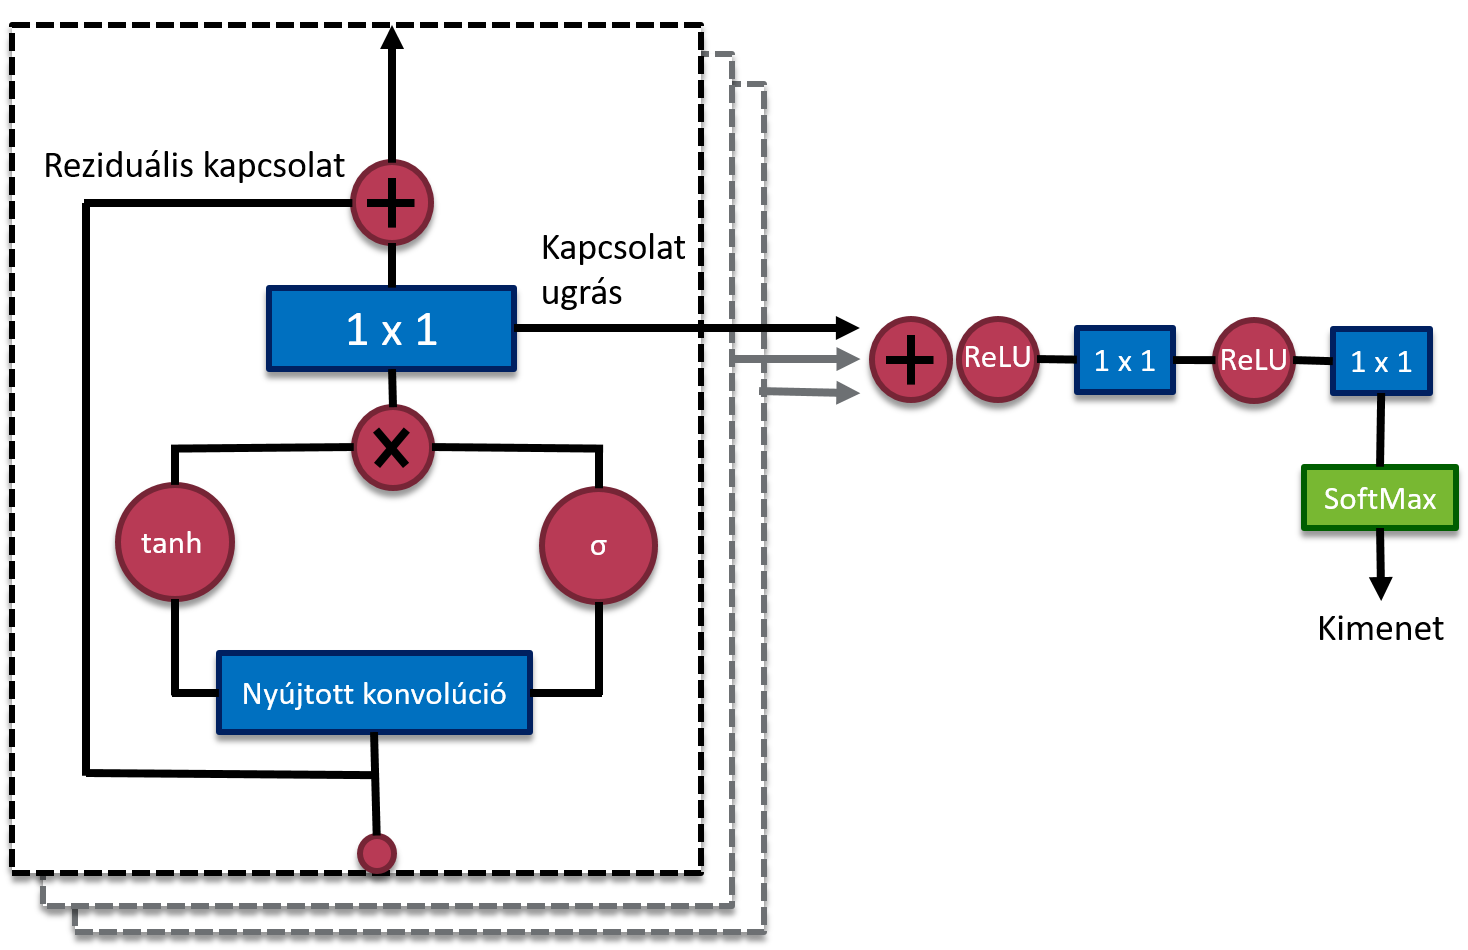
\includegraphics[width=150mm, keepaspectratio]{figures/wavenet_arch.png}
	\caption{WaveNet architektúra.}
	\label{fig:wavenet_arch}
\end{figure}

Egy reziduális blokk bemenete egy 2x1-es konvolúciós rétegen megy keresztül. Balra egy \emph{tanh}, jobbra egy szigmoid aktivációs függvényen haladnak át, majd elemenkénti szorzás és 1x1 konvolúció után egyrészt átugorja a reziduális kapcsolatot, illetve azzal együtt bemenetként szolgál a következő reziduális egységnek. Az 1x1 konvolúciós rétegek a dimenzionalitás változtatására szolgál. Külön 1x1 konvolúciós szűrők skálázzák a kimenetet a következő reziduális blokk bemenetére, és a kapcsolat-ugrásokhoz.

\subsection{Módosított WaveNet architektúra}

A módosított WaveNet architektúra segítségével a WaveNetet beszélőfelismerésre használhatjuk.
\bigskip
\begin{python}
	from WaveNetClassifier import WaveNetClassifier
	
	wnc = WaveNetClassifier((96000,), (10,), kernel_size = 2, dilation_depth = 9,
	                         n_filters = 40, task = 'classification')
	
	wnc.fit(X_train, y_train, validation_data = (X_val, y_val), epochs = 100,
	        batch_size = 32, optimizer='adam', save=True, save_dir='./')
	
	y_pred = wnc.predict(X_test)
	
\end{python}
\bigskip
A WaveNetClassifier objektum paraméterei:

\begin{itemize}
	\item \emph{input\_shape}: Bemeneti dimenziók tuple formájában. Például ha a bemenet egy 6 s hosszú hullámforma 16 kHz-en mintavételezve, a bemeneti dimenziók (96000,)
	\item \emph{output\_shape}: Kimeneti dimenziók tuple formájában. Például ha 100 osztály szerint klasszifikálunk, a kimeneti dimenziókból képzett tuple (100,).
	\item \emph{kernel\_size}: A konvolúciós filter/kernel mérete a reziduális blokkokban.
	\item \emph{dilation\_depth}: A reziduális blokkok száma.
	\item \emph{n\_filters}: A konvolúciós filterek száma a reziduális blokkokban.
	\item \emph{task}: Klasszifikáció vagy regresszió.
	\item \emph{regression\_range}: A regresszió céltartománya lista vagy tuple formátumban.
	\item \emph{load}: Előző WaveNetClassifier betöltése (bool).
	\item \emph{load\_dir}: A betölteni kívánt modell könyvtára.
\end{itemize}

\subsection{Eredmények}

A WaveNet classifiert mindkét beszédadatbázison teszteltem. A TIMIT beszédkorpusszal csak kevés beszélő esetén ért el jó eredményt, több mint 20 beszélő esetén a modell nem tanult. Ennek valószínűsített oka, hogy a TIMIT adatbázis beszélőnként 10 hangmintát tartalmaz.

\setlength\arrayrulewidth{0.6pt}

\begin{table}[!ht]
	\begin{tabular}{l|l} \toprule
		\bfseries Beszélők száma & 18 \\
		\rowcolor{gray!10}
		\bfseries Minta/beszélő & 100\\
		\bfseries Minta össz. & 1800 \\
		\rowcolor{gray!10}
		\bfseries Minta hossza & 4000 \\
		\bfseries Epochok száma & 43\\
		\rowcolor{gray!10}
		\bfseries Hiba & 0.0013 \\ 
		\bfseries Pontosság & 1.0 \\ 
		\bottomrule
		\hline
	\end{tabular}
	\centering
	\caption{Paraméterek CMU Arctic adatbázissal.}
	\label{fig:wavenet-arctic}
\end{table}

!!! teszthalmaz mérete !!!

Tanítás után a teszt adathalmazon a hálózat 96.799 \%-os pontosságot ért el.

\section{SincNet}



\subsection{Eredmények}